% https://www.overleaf.com/learn/latex/Beamer#Introduction
% https://en.wikibooks.org/wiki/LaTeX/Presentations#The_Beamer_package
\documentclass{beamer}
\usepackage[utf8]{inputenc}
% http://texblog.net/latex-archive/latex-general/beamer-warnings/
\usepackage{lmodern}
% https://hartwork.org/beamer-theme-matrix/
% \usecolortheme{dove}

% https://tex.stackexchange.com/a/356169
\usepackage[style=ieee,backend=bibtex]{biblatex}
\addbibresource{bibliography.bib}

\beamertemplatenavigationsymbolsempty
% https://tex.stackexchange.com/a/74251
\setbeamerfont{page number in head/foot}{size=\small}
\setbeamertemplate{footline}[frame number]
\setbeamerfont{footnote}{size=\tiny}
 
\author{Russel Shawn Dsouza}
% https://tex.stackexchange.com/a/61053
\institute
{
  
\includegraphics[scale=0.25]{images/logo}\\
  Electronics and Communications Engg.\\
  National Institute of Technology Karnataka\\
  Surathkal, India - 575025
}
\date{February 28, 2020}

\title[Sparsity]{Sparse neural networks}
 
\begin{document}

  % https://stackoverflow.com/a/54916411
  \begingroup
    \setbeamertemplate{footline}{}
    \frame{\titlepage}
  \endgroup

  \addtocounter{framenumber}{-1}

  % https://tex.stackexchange.com/a/198102
  \begin{frame}{Overview}
    \tableofcontents
  \end{frame}

  \section{Motivation for sparsity}
  \begin{frame}
    \frametitle{Motivation for sparsity: Network Theory}
    Fewer links than the maximum possible links\\
    Ex: Social and computer networks
    \begin{figure}
        \centering
        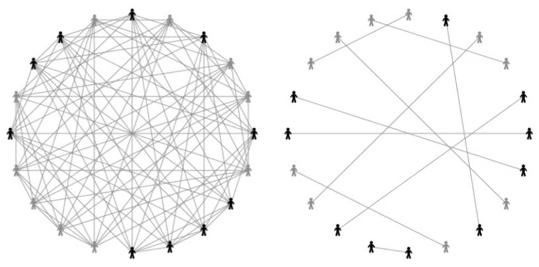
\includegraphics[width=.7\textwidth]{images/social_network.jpg}
        \caption{Dense vs Sparse social networks\footfullcite{sparse_social_network}}
    \end{figure}
  \end{frame}
  
  \begin{frame}
    \frametitle{Motivation for sparsity: Deep Learning (-1998)}
    \begin{figure}
        \centering
        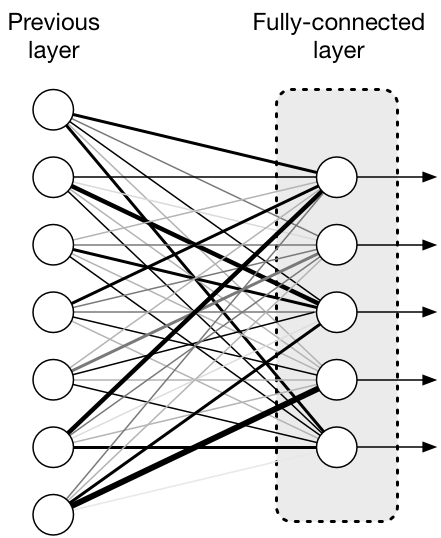
\includegraphics[width=.4\textwidth]{images/fully_connected.png}
        \caption{Fully connected networks\footfullcite{fukushima1988neocognitron}}
    \end{figure}
  \end{frame}
  
  \begin{frame}
    \frametitle{Motivation for sparsity: Deep Learning (-2019)}
    \begin{figure}
        \centering
        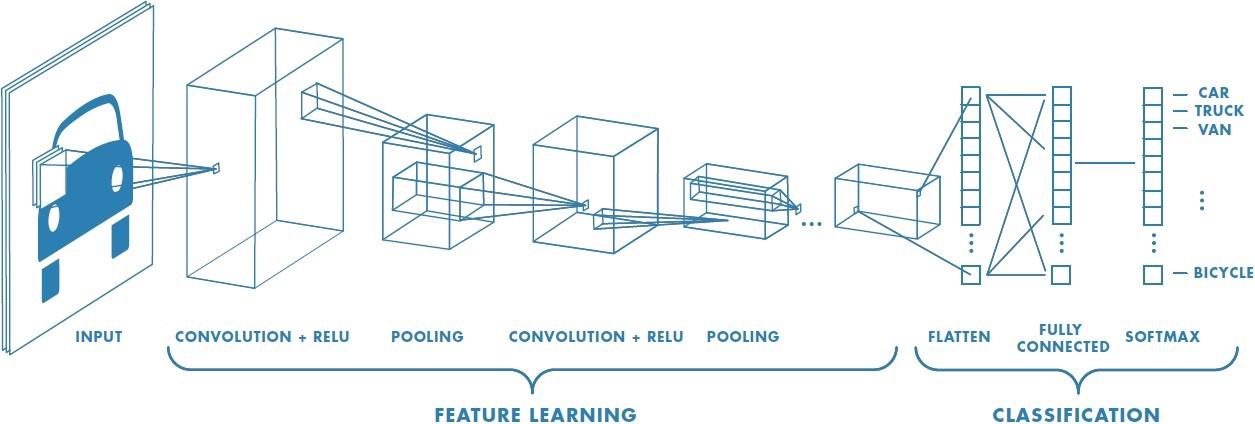
\includegraphics[width=\textwidth]{images/cnn.jpeg}
        \caption{Convolutional neural network\footfullcite{cnn_eli5}}
    \end{figure}
  \end{frame}
 
  \begin{frame}
    \frametitle{Motivation for sparsity: Neocortex}
    \begin{figure}
        \centering
        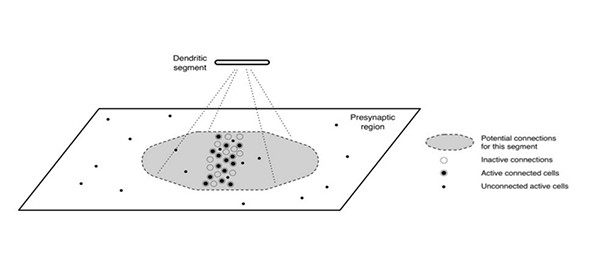
\includegraphics[width=\textwidth]{images/sparse-brain.png}
        \caption{Sparse coding in the brain\footfullcite{sparse_brain_numenta}}
    \end{figure}
  \end{frame}
  
  
  \section{Sparsity in neural networks}
  \begin{frame}
      \frametitle{Sparsely connected layers}
      \begin{figure}
        \centering
        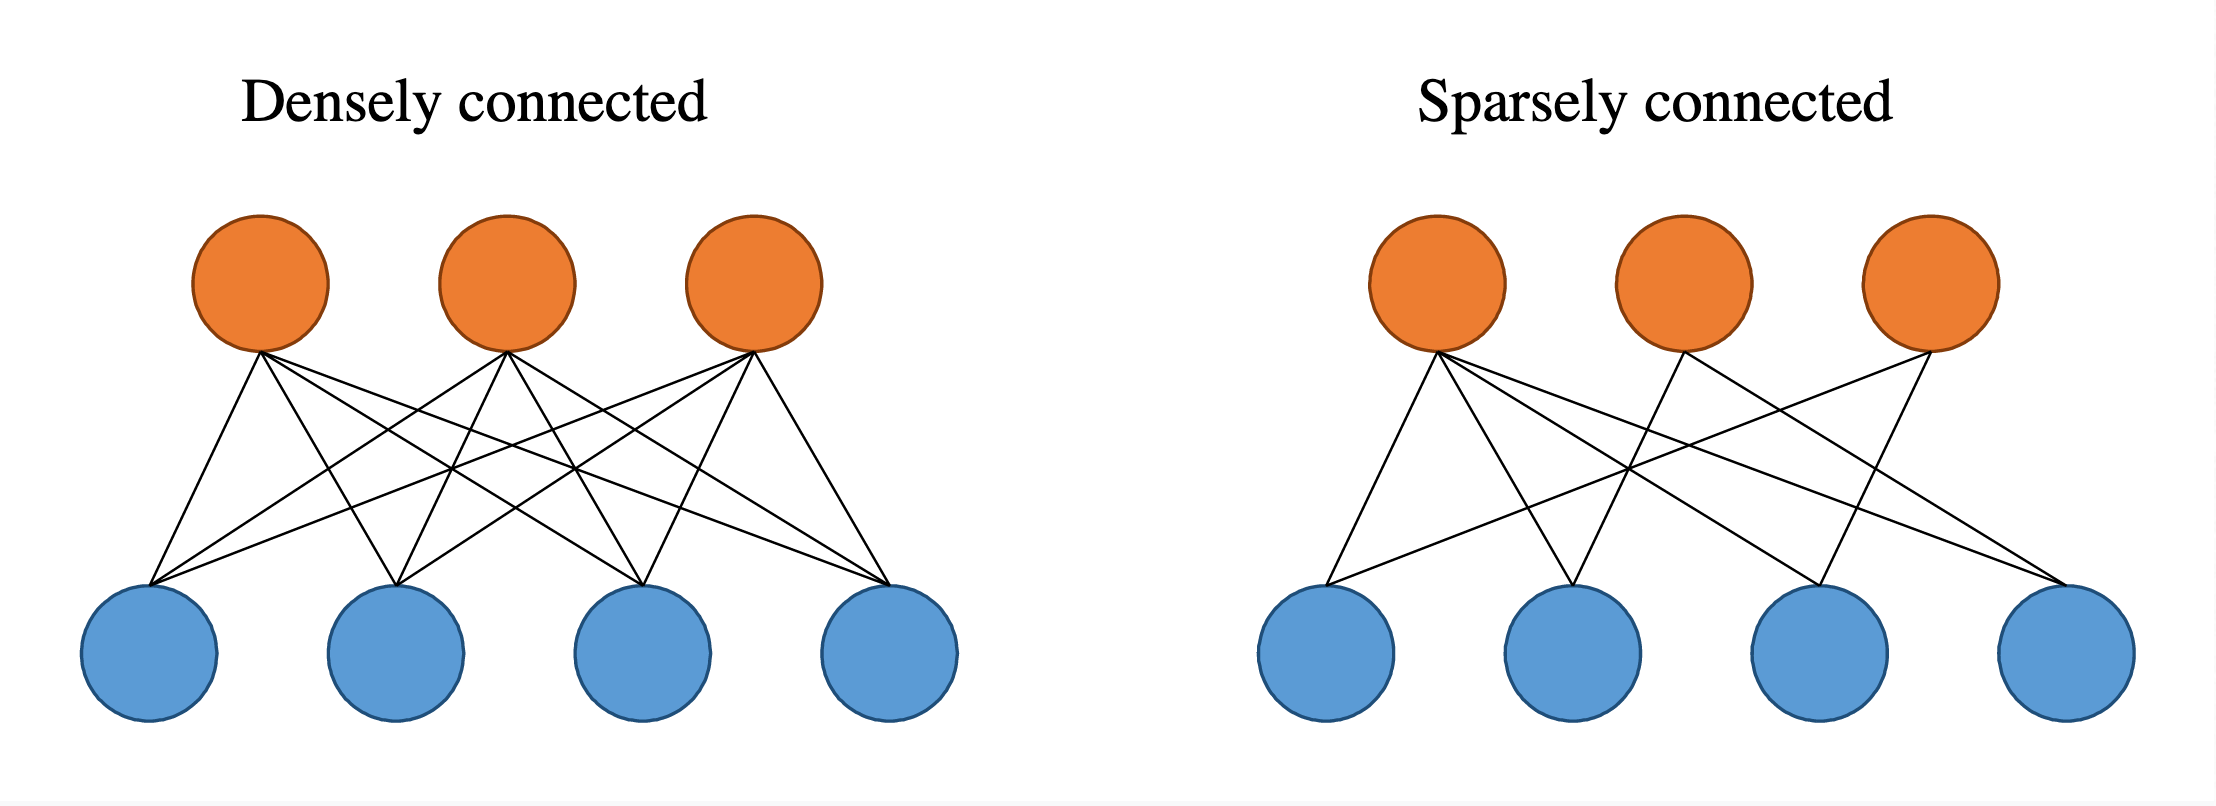
\includegraphics[width=\textwidth]{images/sparse_vs_dense.png}
        \caption{Dense vs Sparse networks\footfullcite{sparse_vs_dense}}
    \end{figure}
  \end{frame}
  
  
  \begin{frame}
    \frametitle{How to learn connections?}
    \textbf{Observed networks in data source}\\
    \begin{figure}
      \centering
      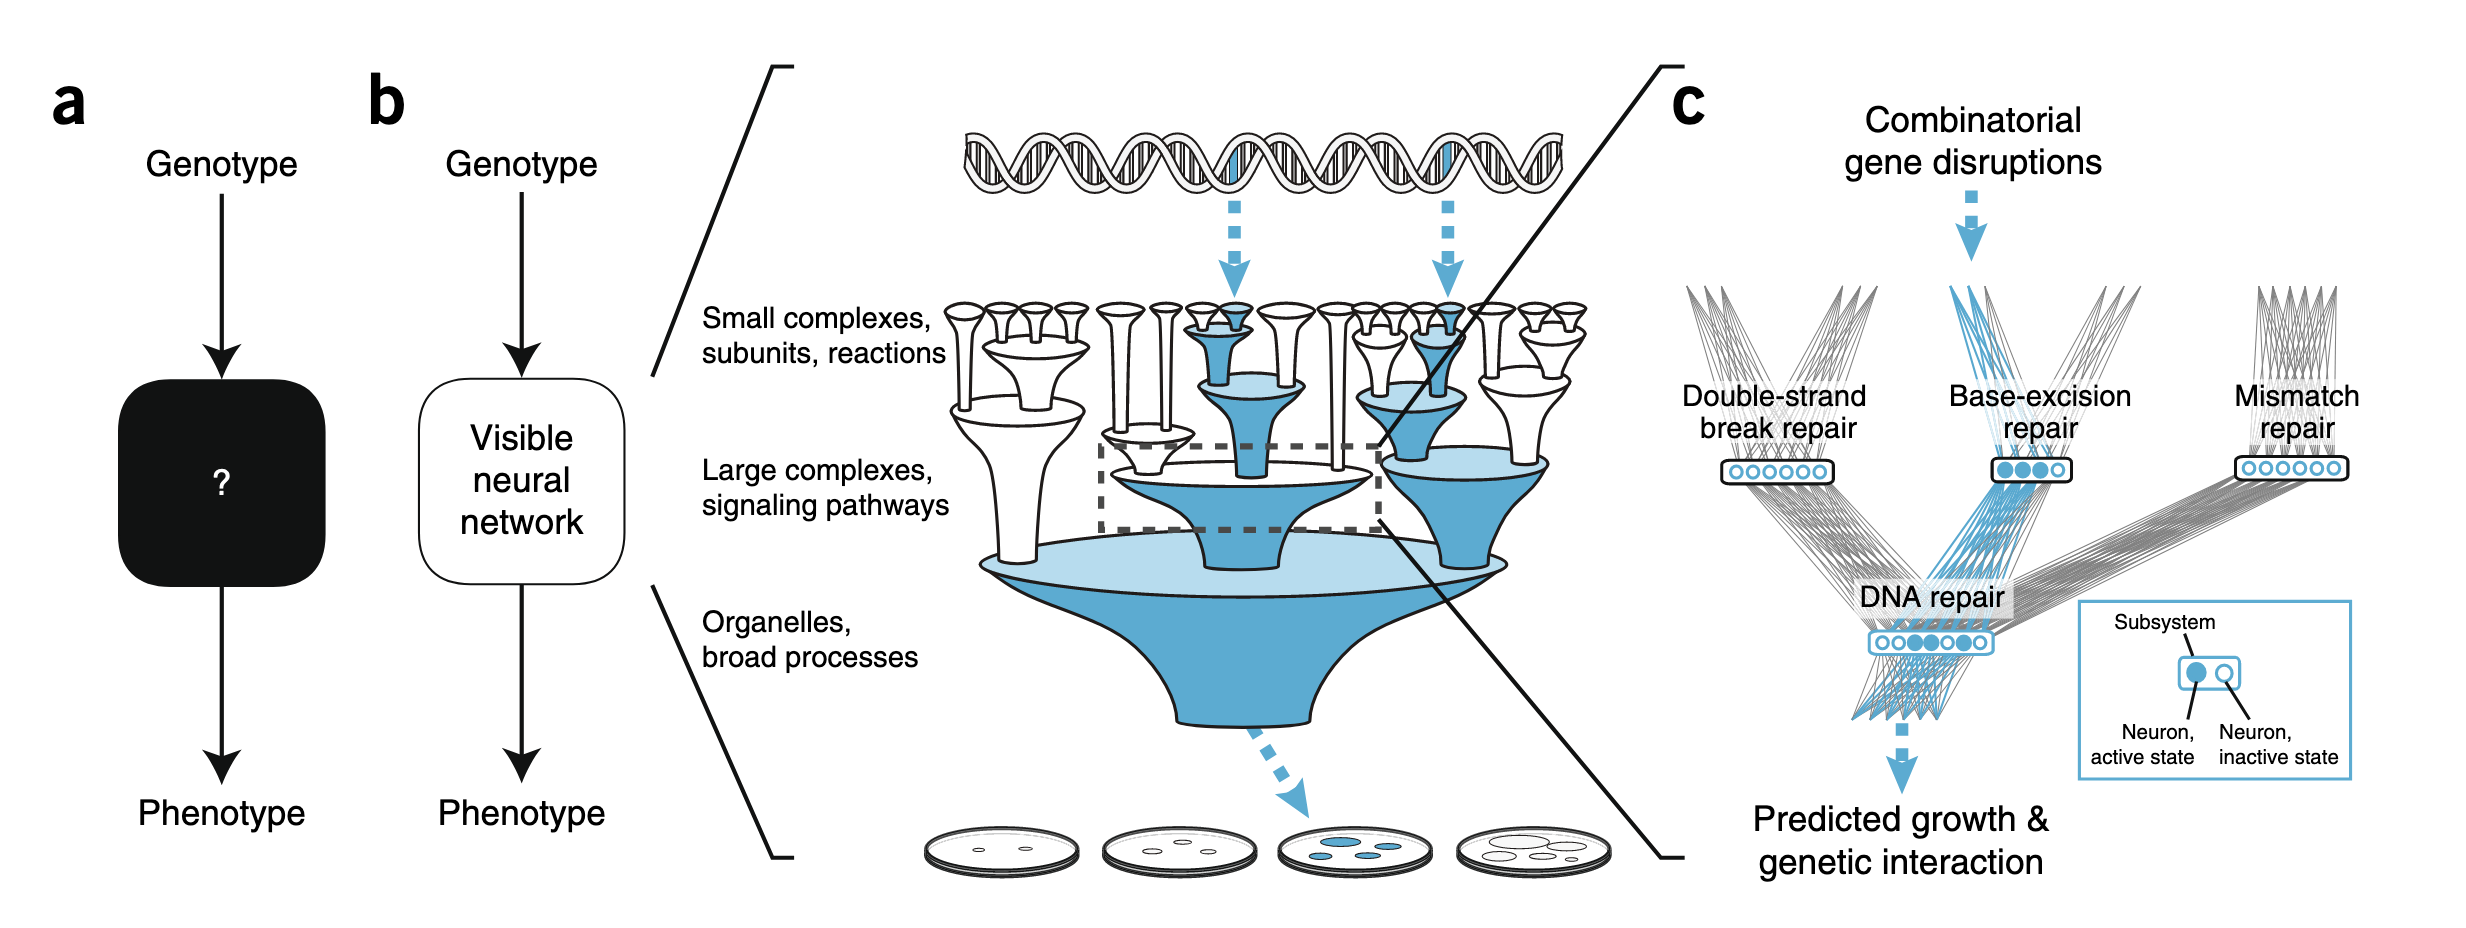
\includegraphics[width=\textwidth]{images/vnn.png}
      \caption{Protein interaction networks\footfullcite{ma2018using}}
    \end{figure}
  \end{frame}
  
  \begin{frame}
    \frametitle{How to learn connections?}
    \textbf{Pruning\footfullcite{han2015learning}}\\
    \begin{columns}
        \column{.3\textwidth}
        \begin{figure}
            \centering
            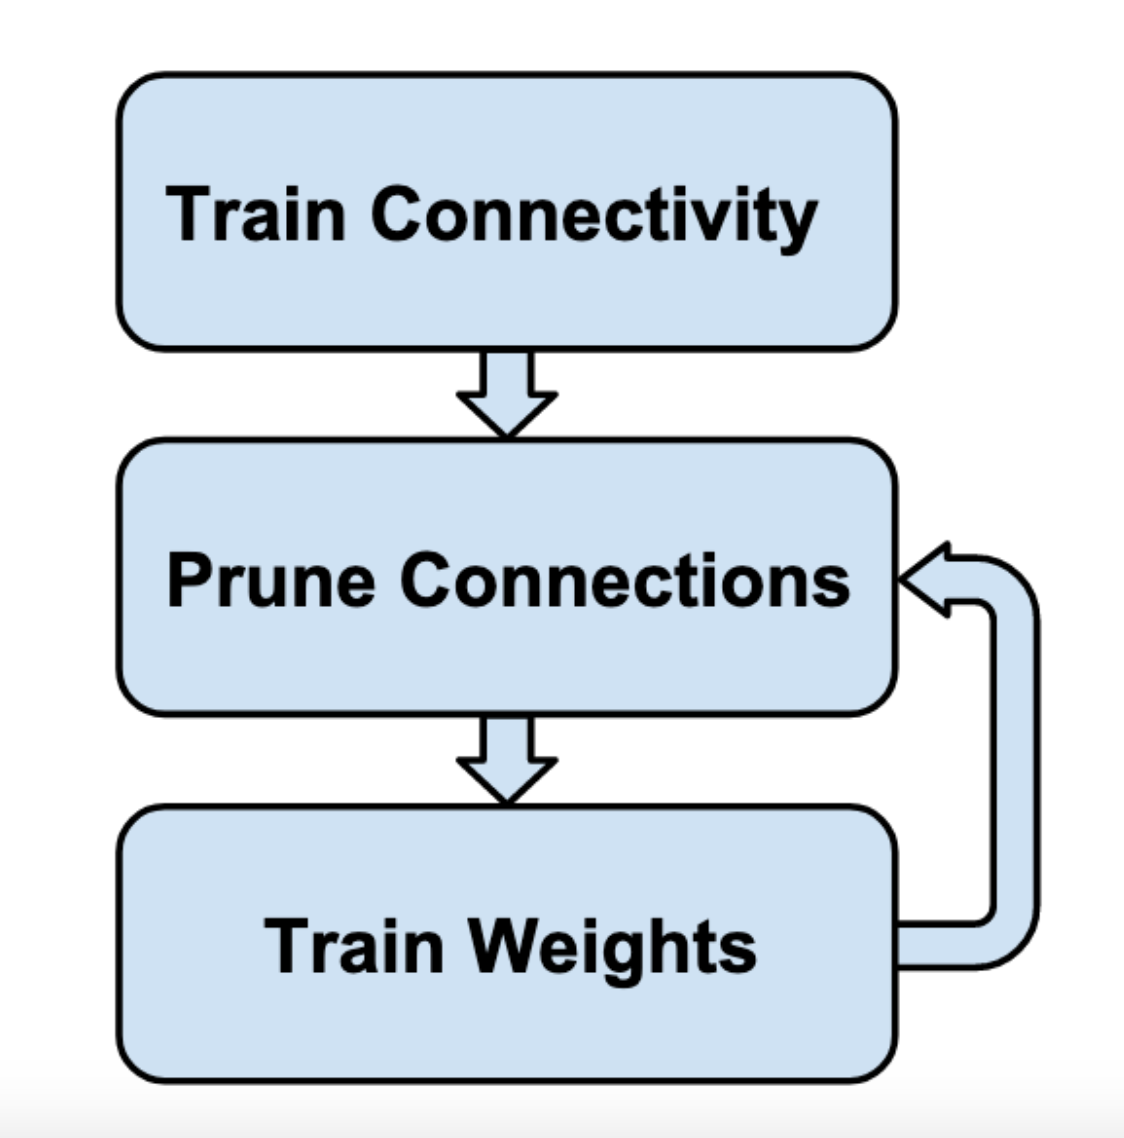
\includegraphics[width=\textwidth]{images/pruning_pipeline.png}
            \caption{The three step pipeline}
        \end{figure}
        \column{.5\textwidth}
        \begin{figure}
            \centering
            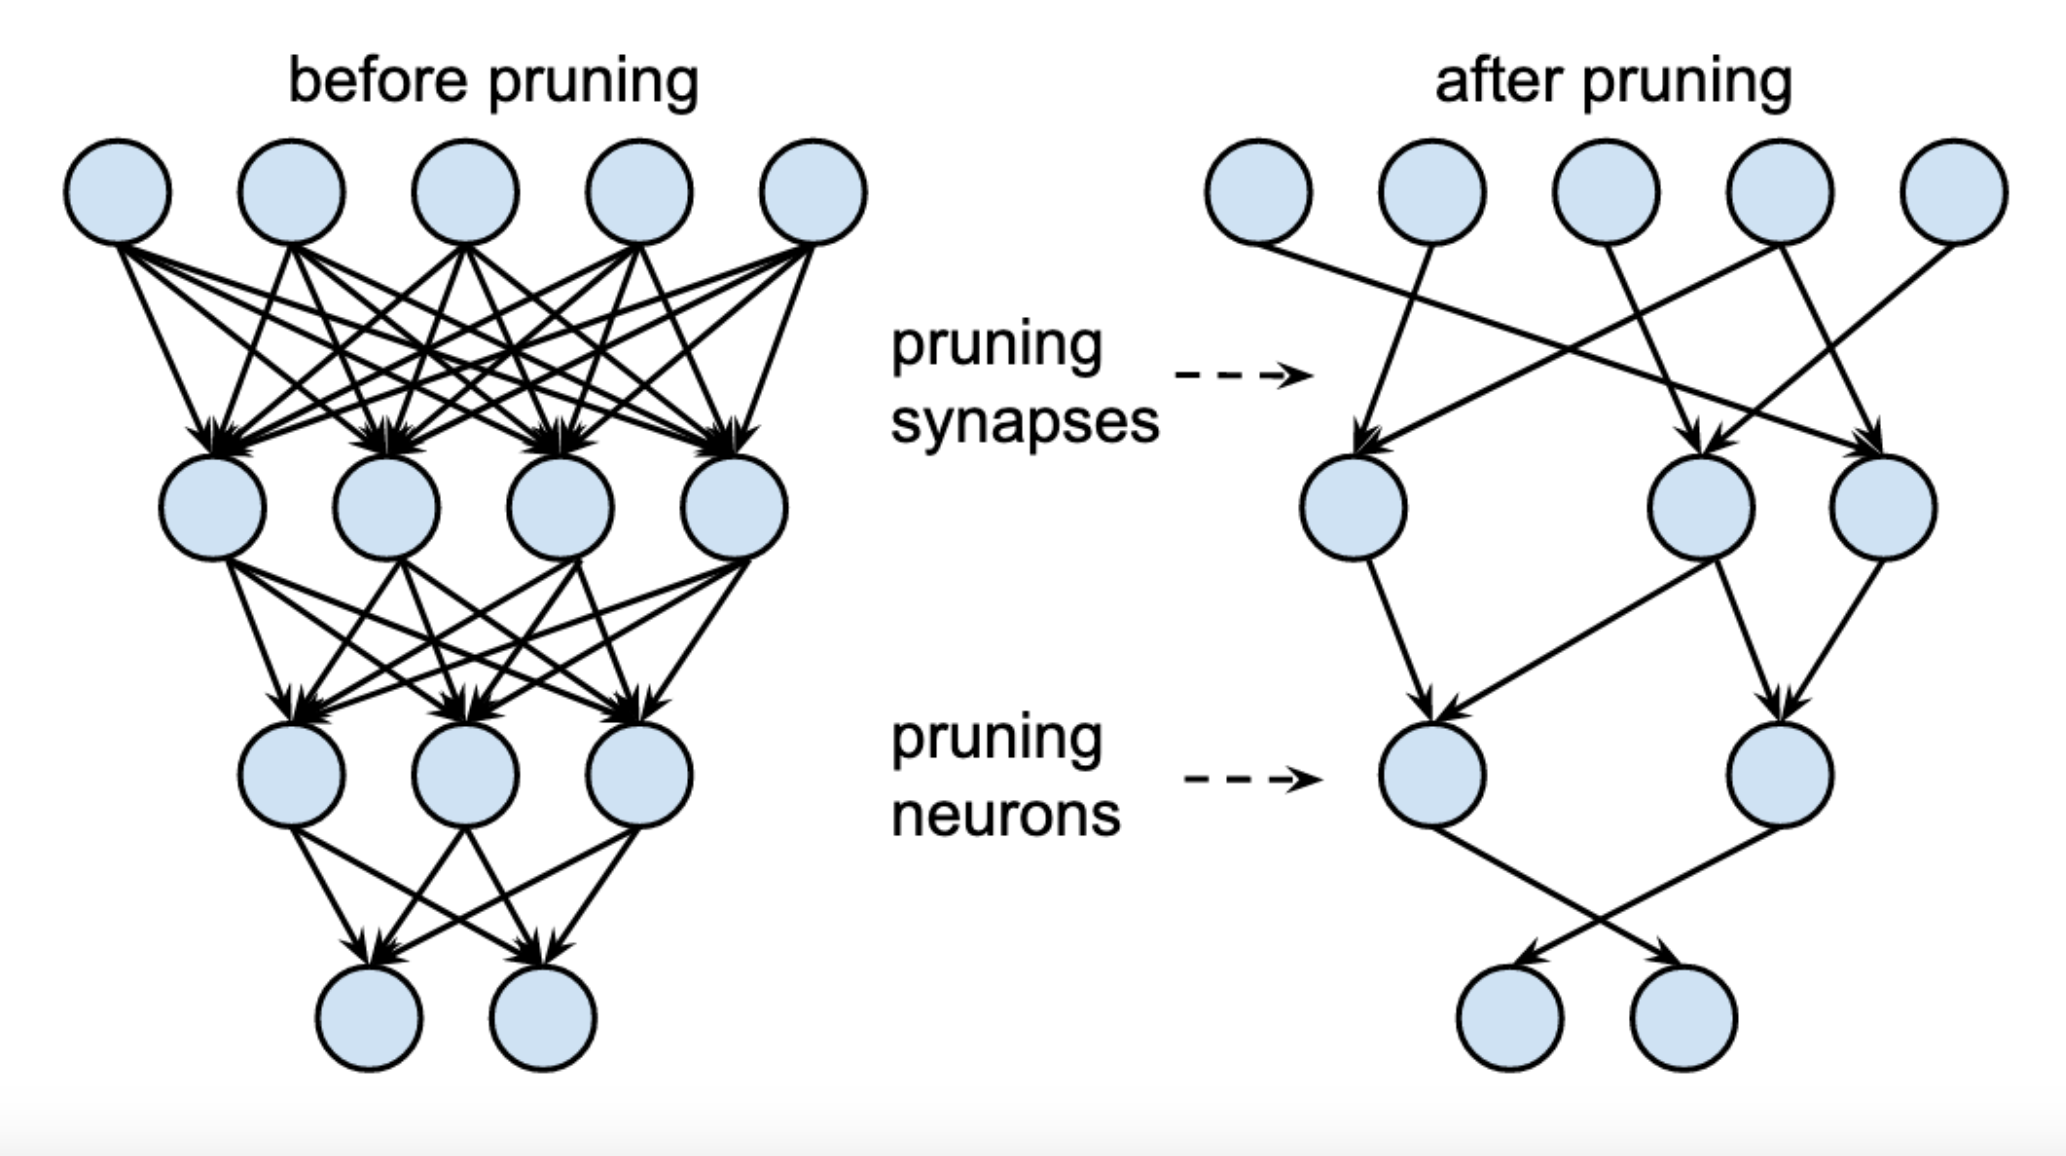
\includegraphics[width=\textwidth]{images/pruning_before_and_after.png}
            \caption{Pruning: before and after}
        \end{figure}
    \end{columns}
  \end{frame}
  
  \begin{frame}
    \frametitle{How to learn connections?}
    \textbf{Adaptive sparse connectivity}
    \begin{figure}
        \centering
        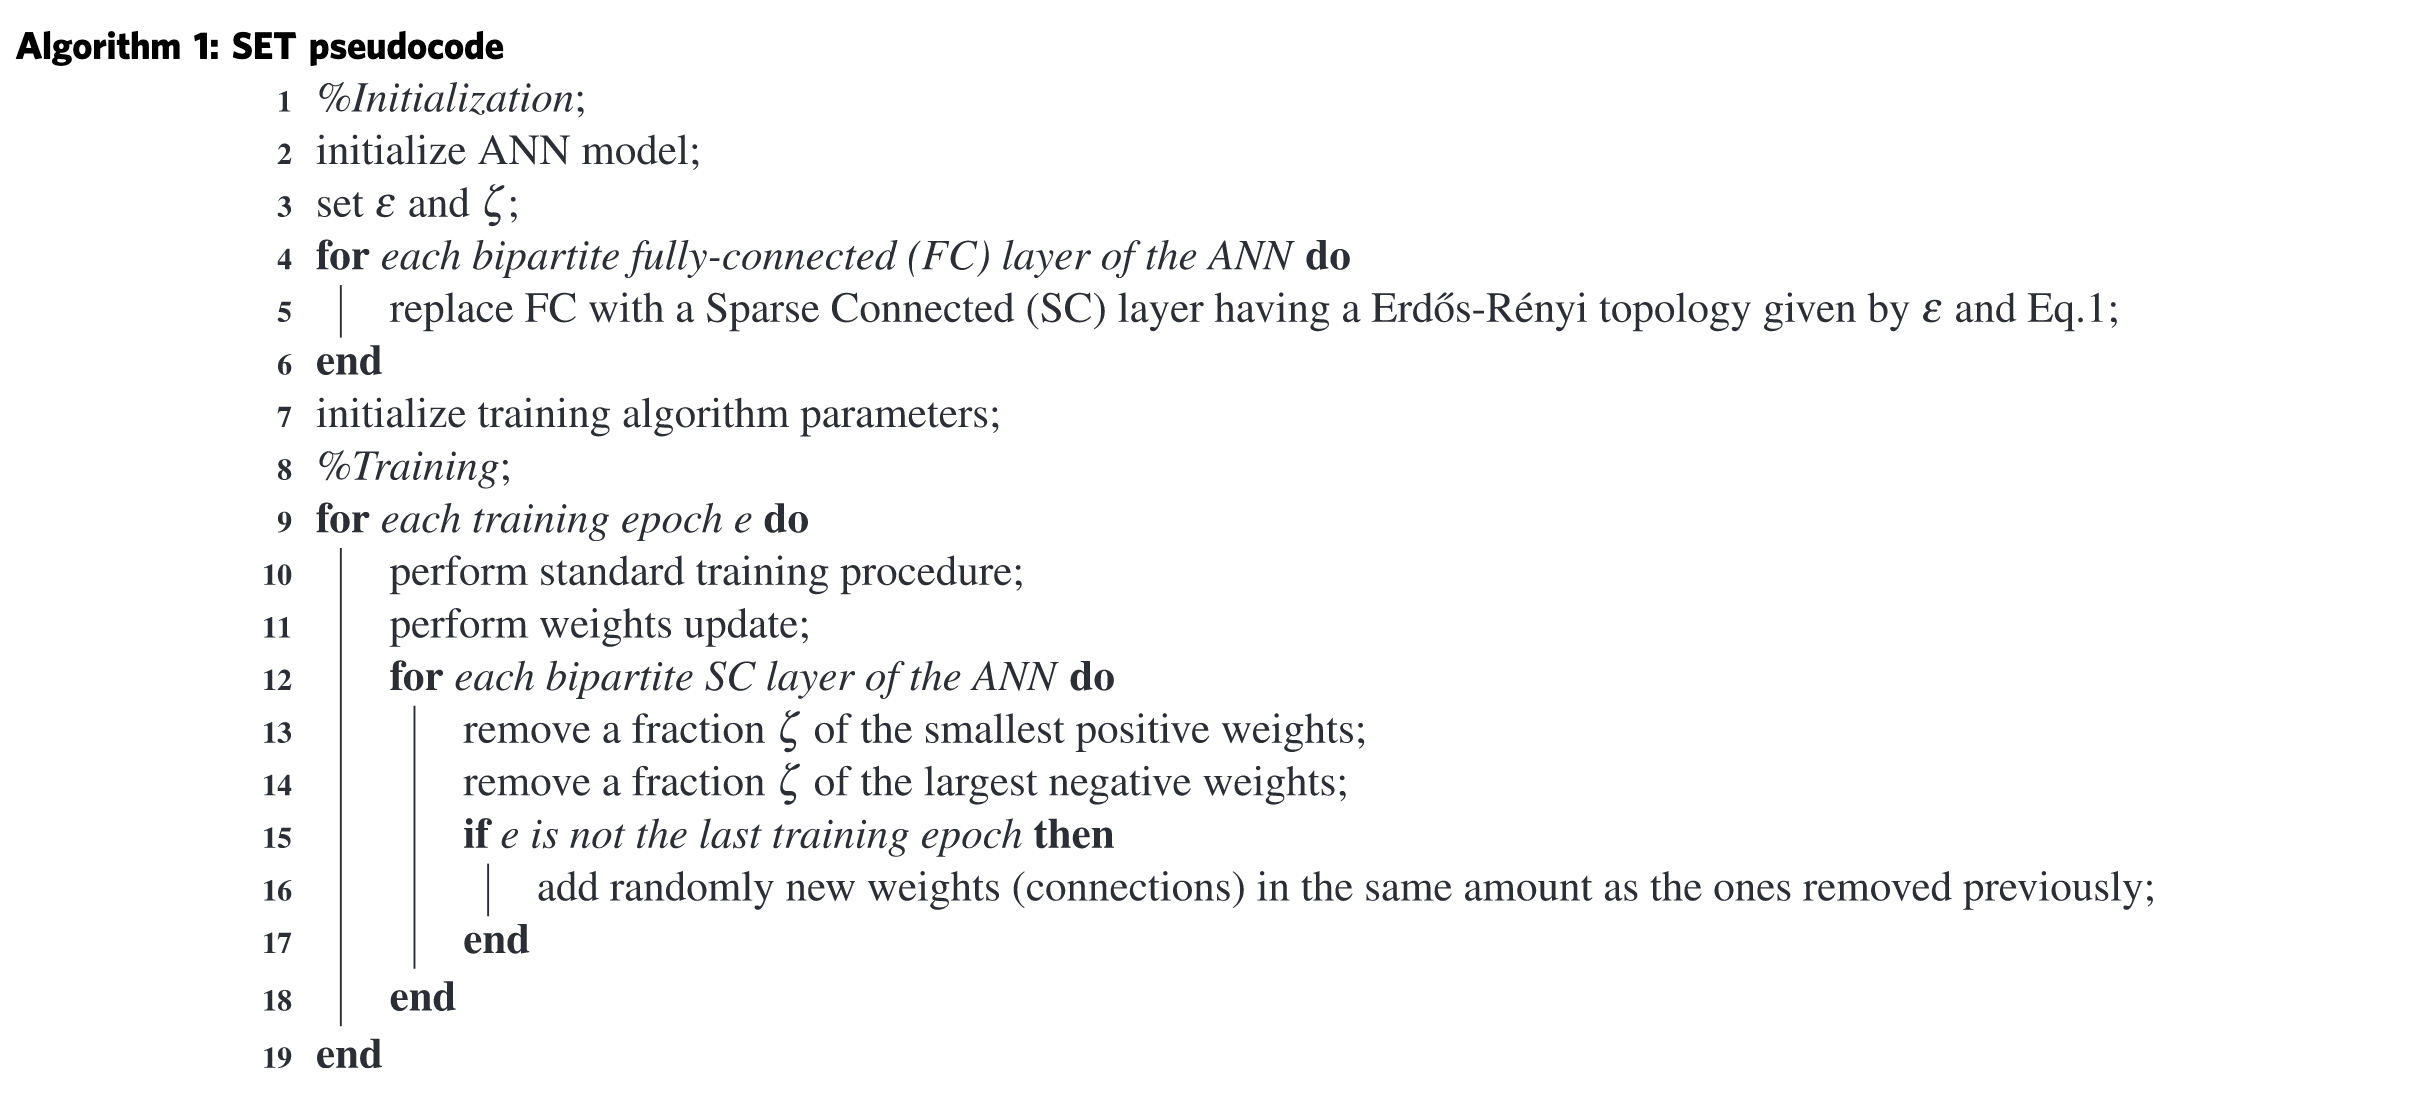
\includegraphics[width=\textwidth]{images/set_algo.png}
        \caption{Sparse Evolutionary Training (SET) algorithm\footfullcite{mocanu_scalable_2018}}
    \end{figure}
  \end{frame}
  
  \begin{frame}
    \frametitle{SET: Encoding domain-specific information}
    \begin{figure}
        \centering
        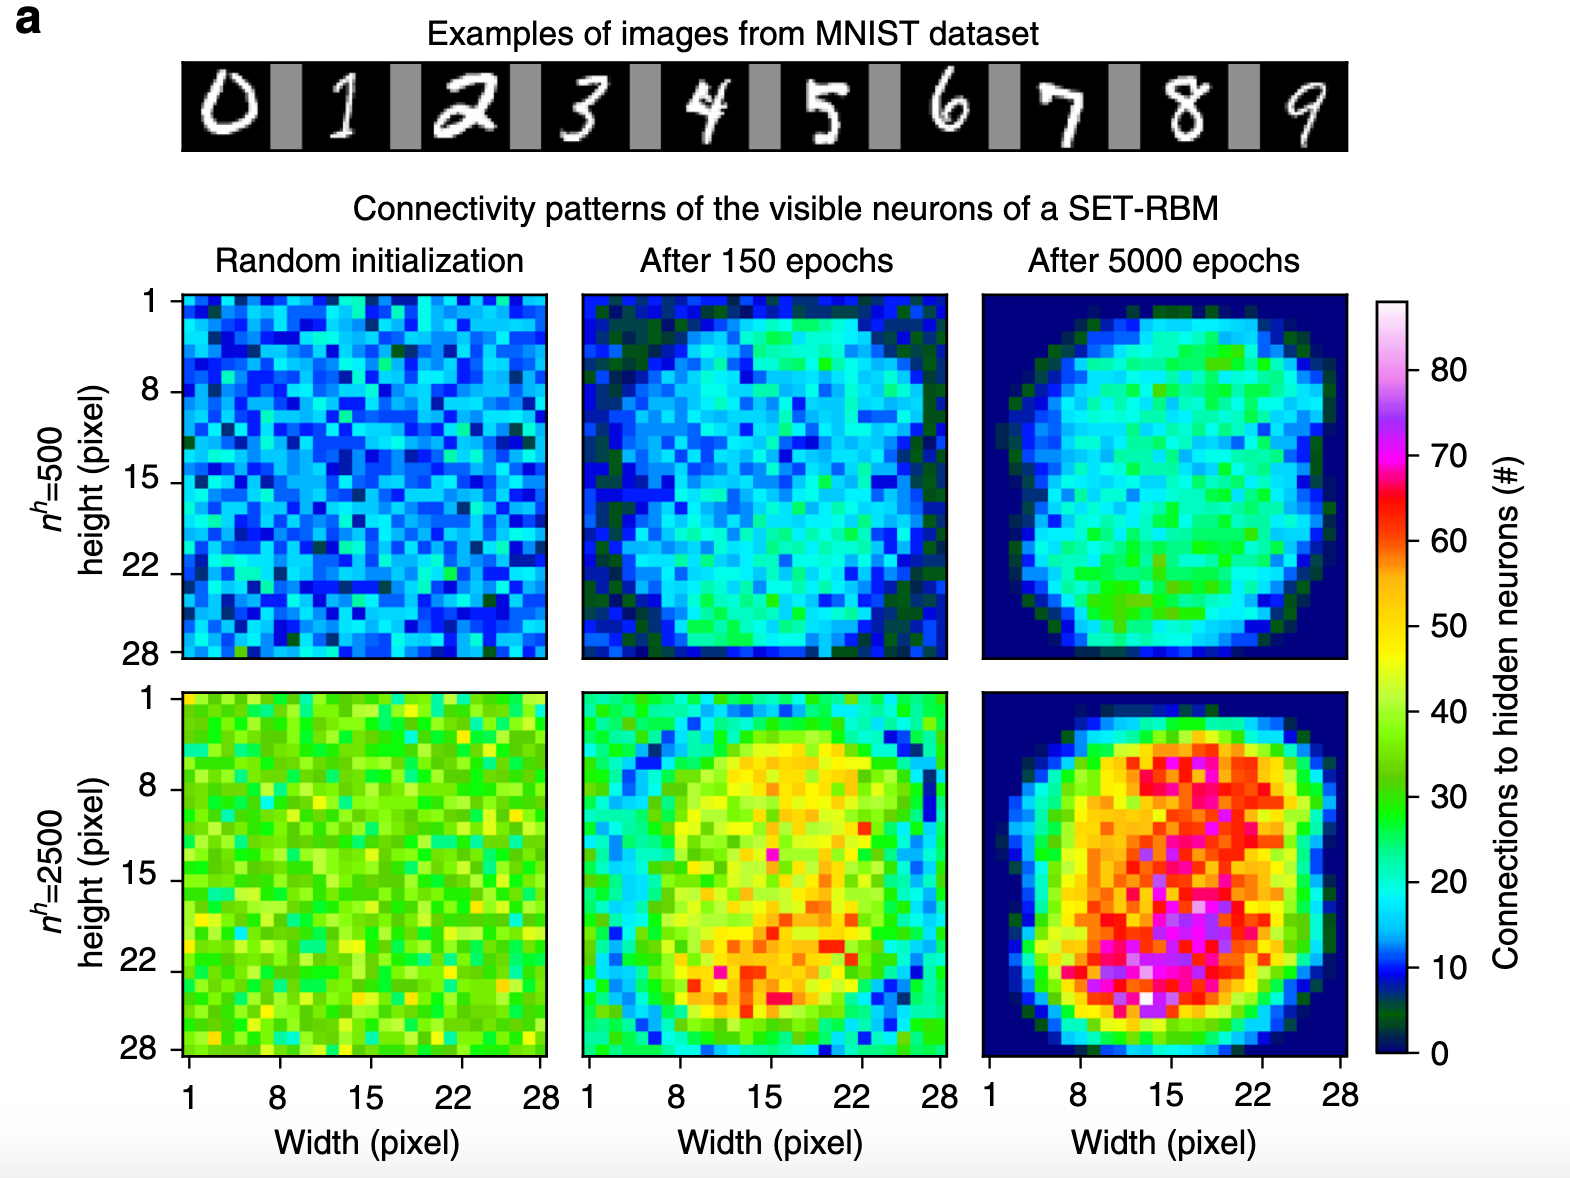
\includegraphics[width=.7\textwidth]{images/mnist_scl.png}
        \caption{Input connections of an SET trained on MNIST \footfullcite{mocanu_scalable_2018}}
    \end{figure}
  \end{frame}

  
  \section{Advantages}
  \begin{frame}
    \frametitle{Advantages}
    \begin{itemize}
        \item Robustness \footfullcite{ahmad2016neurons}
        \item Better fit to lifelong learning \footfullcite{cui2016continuous}
        \item Task specific sub-networks \footfullcite{golkar2019continual}
        \item Help discover relationships in unstructured data\footfullcite{mocanu_scalable_2018}
    \end{itemize}
  \end{frame}
  
  
  \section{Research directions}
  \begin{frame}
    \frametitle{Research directions}
    \begin{itemize}
        \item Outperform dense models, but start by training dense models
        \item Sparse matrix multiplications limited in performance\footfullcite{changpinyo2017power}
    \end{itemize}
  \end{frame}


  \begin{frame}
    \frametitle{References}
    \begin{enumerate}
      \item \fullcite{mocanu_scalable_2018}
      \item \fullcite{numenta_sparse_pruning}
      \item \fullcite{klear_sparse_2018}
    \end{enumerate}
  \end{frame}

\end{document}
